Zwei Körper A und B starten zur Zeit $t = 0$ am selben Ort auf einer geraden Linie. Das Diagramm zeigt ihre Geschwindigkeiten.
\begin{center}
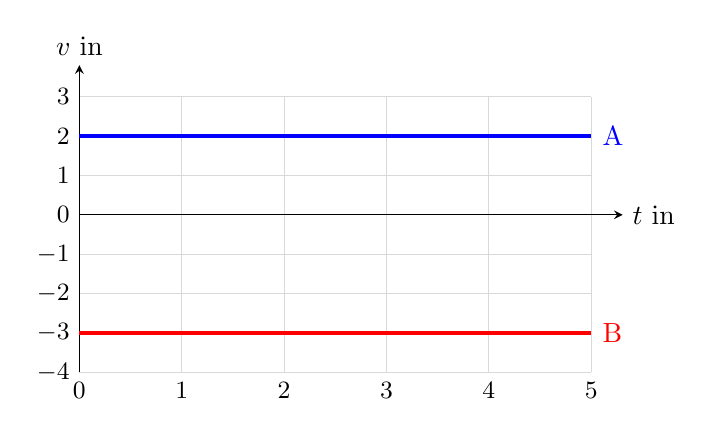
\begin{tikzpicture}[>=stealth, x=1.3cm, y=0.5cm]
 \draw[gray!30] (0,-4) grid[xstep=1, ystep=1] (5,3);
 \draw[->] (0,0) -- (5.308,0) node[right] {$t$ in \si{\second}};
 \draw[->] (0,-4) -- (0,3.8) node[above] {$v$ in \si{\meter\per\second}};
 \foreach \tk in {0,1,2,3,4,5} \node[below] at (\tk,-4) {\small $\tk$};
 \foreach \yk in {-4,-3,-2,-1,0,1,2,3} \node[left] at (0,\yk) {\small $\yk$};

 \draw[ultra thick, blue] (0,2) -- (5,2) node[right] {A};
 \draw[ultra thick, red] (0,-3) -- (5,-3) node[right] {B};
\end{tikzpicture}
\end{center}
\begin{abcliste}
\abc Welcher Körper ist zur Zeit \tEO\ weiter vom Startort entfernt?
\abc Wie weit sind A und B dann voneinander entfernt?
\end{abcliste}
